\section{501 --- Find Mode in Binary Search Tree}
Given a binary search tree (BST) with duplicates, find all the mode(s) (the most frequently occurred element) in the given BST.

Assume a BST is defined as follows:

\begin{itemize}
\item The left subtree of a node contains only nodes with keys less than or equal to the node's key.
\item The right subtree of a node contains only nodes with keys greater than or equal to the node's key.
\item Both the left and right subtrees must also be binary search trees.
\end{itemize}
 
\paragraph{Example:}

\begin{flushleft}
\textbf{Input}:
\begin{figure}[H]
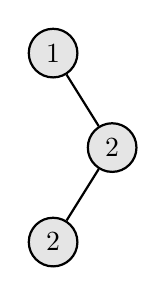
\begin{tikzpicture}
[level distance=12mm, every node/.style={draw, circle,minimum size=6mm, fill=gray!20!},thick]
\node{1}
	child[missing]
	child{node{2} child{node{2}} child[missing]};
\end{tikzpicture}
\end{figure}
\textbf{Output}: 2
\end{flushleft}

\paragraph{Note:} 

\begin{itemize}
\item If a tree has more than one mode, you can return them in any order.
\end{itemize}

\paragraph{Follow up:} 
\begin{itemize}
\item Could you do that without using any extra space? (Assume that the implicit stack space incurred due to recursion does not count).
\end{itemize}

\subsection{Inorder Traverse}
\begin{itemize}
\item 由于是BST,因此inorder遍历的结果是递增序列
\item 这样问题就转换成在递增序列中寻找连续的相同值的个数。
\end{itemize}

\setcounter{lstlisting}{0}
\begin{lstlisting}[style=customc, caption={Inorder Traverse}]
vector<int> findMode( TreeNode* root )
{
    if( !root )
    {
        return {};
    }

    int count = 0;
    int max_count = 0;

    //since at first, count is 1
    //so set last to root-val is safe
    int last = root->val;

    vector<int> ans;

    inorder( root, last, count, max_count, ans );

    return ans;
}

//inorder traverse
void inorder( TreeNode* node, int& last, int& count, int& max_count, vector<int>& modes )
{
    if( !node )
    {
        return;
    }

    inorder( node->left, last, count, max_count, modes );

    if( node->val != last )
    {
        last = node->val;
        count = 1;
    }
    else
    {
        ++count;
    }

    if( count > max_count )
    {
        //new maximum count
        max_count = count;
        //remove all elements in modes
        modes.clear();
        modes.push_back( node->val );
    }
    else if( count == max_count )
    {
        //new element that has maximum count
        modes.push_back( node->val );
    }

    inorder( node->right, last, count, max_count, modes );
}
\end{lstlisting}